% Nicholas Arnold
% Steven Braeger
% COP 6616
%
% Project Progress Report
%
% We used the template from IEEE website, linked from
% http://www.ieee.org/conferences_events/conferences/publishing/templates.html	

\documentclass[conference]{IEEEtran}

% *** CITATION PACKAGES ***
%
%\usepackage{cite}
% cite.sty was written by Donald Arseneau
% V1.6 and later of IEEEtran pre-defines the format of the cite.sty package
% \cite{} output to follow that of IEEE. Loading the cite package will
% result in citation numbers being automatically sorted and properly
% "compressed/ranged". e.g., [1], [9], [2], [7], [5], [6] without using
% cite.sty will become [1], [2], [5]--[7], [9] using cite.sty. cite.sty's
% \cite will automatically add leading space, if needed. Use cite.sty's
% noadjust option (cite.sty V3.8 and later) if you want to turn this off.
% cite.sty is already installed on most LaTeX systems. Be sure and use
% version 4.0 (2003-05-27) and later if using hyperref.sty. cite.sty does
% not currently provide for hyperlinked citations.
% The latest version can be obtained at:
% http://www.ctan.org/tex-archive/macros/latex/contrib/cite/
% The documentation is contained in the cite.sty file itself.

% *** MATH PACKAGES ***
%
%\usepackage[cmex10]{amsmath}
% *** SPECIALIZED LIST PACKAGES ***
%
%\usepackage{algorithmic}
% algorithmic.sty was written by Peter Williams and Rogerio Brito.
% This package provides an algorithmic environment fo describing algorithms.
% You can use the algorithmic environment in-text or within a figure


% *** ALIGNMENT PACKAGES ***
%
%\usepackage{array}
%\usepackage{mdwmath}
%\usepackage{mdwtab}
%\usepackage{eqparbox}

% *** SUBFIGURE PACKAGES ***
%\usepackage[tight,footnotesize]{subfigure}

%\usepackage[caption=false]{caption}
%\usepackage[font=footnotesize]{subfig}
%\usepackage{fixltx2e}
%\usepackage{stfloats}
% stfloats.sty was written by Sigitas Tolusis. This package gives LaTeX2e
% the ability to do double column floats at the bottom of the page as well
% as the top. (e.g., "\begin{figure*}[!b]" is not normally possible in
% LaTeX2e). It also provides a command:
%\fnbelowfloat
% to enable the placement of footnotes below bottom floats (the standard
% LaTeX2e kernel puts them above bottom floats). This is an invasive package

% Other Packages
\usepackage{moreverb}
\usepackage{graphicx}
\usepackage{caption}
\usepackage{url}

% correct bad hyphenation here
\hyphenation{op-tical net-works semi-conduc-tor}


\begin{document}
%
% paper title
% can use linebreaks \\ within to get better formatting as desired
\title{Scalable N-Body Event Prediction}


% author names and affiliations
% use a multiple column layout for up to three different
% affiliations
\author{\IEEEauthorblockN{Steven Braeger}
\IEEEauthorblockA{Department of Electrical Engineering and\\Computer Science\\
University of Central Florida\\
Orlando, Florida 32826\\
Email: steve@soapforge.com}
\and\IEEEauthorblockN{Nicholas Arnold}
\IEEEauthorblockA{Department of Electrical Engineering and\\Computer Science\\
University of Central Florida\\
Orlando, Florida 32826\\
Email: narnold@knights.ucf.edu}
}

\maketitle


\begin{abstract} %Steven
The general simulation of n-body systems often requires the simulation of pairwise interaction events between the objects.  The naive method of simulating these events is an algorithm that polls each pair of object for an interaction every timestep.  This algorithm has $O(n^2)$ operations per timestep in the number of objects.  However, this method scales very well to multiple cores. In this paper, we propose a novel method of pairwise simulation that saves a significant amount of computation time by predicting possible future outcomes rather than reacting to them.  We demonstrate the implementation of this method, as well as prove that it has amortized $O(n)$ complexity per timestep.  We also demonstrate a lock-free implementation to allow this algorithm to scale comparably to multiple cores of a shared memory machine.
\end{abstract}

\IEEEpeerreviewmaketitle


\section{Introduction}

There is a great deal of interest in discrete event simulation as it applies to video games and real time simulation. One interest in particular is the application of realistic physics in these simulations.  This kind of discrete event simulation is traditionally performed on large scale parallel clusters for film and scientific applications, or on massively parallel GPU architectures \cite{grape,uberflow}.  Specifically, we wish to explore the simulation and evolution of systems of dynamic and static objects where all the dynamic objects interact with all of the other objects, as happens when the dynamic objects physically collide with other objects.  In order to do this, we need to be able to model and react to collisions and interactions between objects. 

Although the naive and semi-naive implementations of this kind of simulation are embarassingly parallel, they are also exceedingly wasteful.  The method used to evaluate the interactions between objects is similar to a busy-wait loop, where all objects are continually polled, waiting for collisions to occur as the simulation progresses \cite{nbodycollisions,Moore88collisiondetection}.   As we will describe in the next sections, we are interested in using a novel predictive model along with a novel lock-free n-body event queue data structure to attempt to make a new kind of economical collision simulation system.  Our hope is that this system does not perform wasteful checks when checks are unlikely and maintains much of the parallelism of the naive solution.

\section{Problem Definition}

As input, we are given a description of static objects, dynamic objects, and the geometry defining their boundaries.  We are also given initial states like position, acceleration and velocity of the objects in the system, and a set of rules to update those objects.  As output, we wish to compute the exact state of each object in the system for each of the $n$ timestamps $t_0, t_1, t_2, \ldots, t_n$.

For each object $o$ in the system, a subroutine is defined \texttt{update($o$,$dt$)}, which computes the state of the object in the next timestamp, given the object state in the current timestamp and a time $dt$ between timestamps.  For each pair of objects $o1$ and $o2$, an additional subroutine is defined \texttt{collide($o1$,$o2$)} which computes the state of both $o1$ and $o2$ in the next timestamp, assuming that the objects have collided during the current timestamp.

\subsection{Naive Algorithm}

The brute force all-pairs solution is the naive solution to this problem as it is commonly implemented in games. This technique is known as a 'detection' technique because it relies on the idea of detecting a collision when it occurs instead of predicting a collision.  

\begin{verbatimtab}[3]
for each timestep ti
	dt is the constant timestep difference
	for each dynamic object "do"
		update(do,dt)		
		for each object  o
			if(check(do,o))
				collide(do, o, dt)
\end{verbatimtab}

This technique is embarassingly parallel, allowing a thread per dynamic object or even a thread per pair with minimal overhead.  However, it is extremely
wasteful, because there are $O(n^2)$ checks being made every single timestamp, even if the likelihood of a collision has changed little since the last timestep \cite{Seningood}.  

Each of these $O(n^2)$ checks per timestep is computationally cheap individually, but when the number of objects is very great the computational overhead of performing all of them becomes
unmanagable. Considering that an extreme majority of the checks will fail due to the fact that collision occurrances are rare, most of them do not need to be computed, and avoiding their computation has the ability to dramatically increase the 
throughput of our simulation.

\subsection{Semi-Naive Algorithm}

A similar algorithm that we refer to as the 'semi-naive' algorithm has also found great use in practical applications \cite{Bittner02hierarchicaltechniques}.  The semi-naive algorithm differs only from the naive algorithm in that it exploits a bounding volume hierarchy to spatially partition the dynamic objects and pre-filter the collision checks.  This algorithm is equally wasteful, but only has $O(n log n)$ checks if the objects are relatively equally distributed throughout the bounding space.

\section{Theoretical Contribution}
\label{sec:theocont}
\subsection{Predictive Algorithm}

In our desired solution, we take a completely different approach.  In contrast to the naive and semi-naive algorithms, our solution avoids computing any unneeded checks on timestamps that do not change the solution by \textit{predicting} the intersections before they occur, rather than checking for them when they do not.  Our algorithm will use a slightly more complex subroutine \texttt{predict($o1$,$o2$)} that returns the time an intersection is likely to occur, and enters it into an event queue that contains the predicted collisions that are likely to occur.  When an intersection occurs, it is recomputed and removed from the queue.

\begin{verbatimtab}[3]
events=future_event_queue()
#initialize events from initial states.

for each timestep ti
	dt is the constant timestep difference
	for each dynamic object "do"
		update(do,dt)

	#for each event that occurs in this timestep
	for each e in events.find(ti) 
		for each object o
			if(check(e.o,o))
				collide(e.o, o, dt)
				#predict next collision event into queue
		events.remove(e)
\end{verbatimtab}

It is worth noting that although our solution is the same runtime complextiy as the naive solution in the worst case (and, in fact, the initial population of event queue will need to preform $n^2$ predictions), it is unlikely to compute ANY checks that are unlikely to occur, thus saving tremendous computation time.  

However, our work is not done.  This algorithm is difficult to parallelize when compared to the naive algorithm, as it depends implicitly on reading and writing the global future nbody event queue data structure described in section \ref{sec:neq}.  This data structure is a specialized queue in which events take priority over other events about to take place. If we split the evaluation of the simulation into threads, then each thread must somehow synchronize which events it will prioritize and avoid collisions.  Furthermore, threads must be able to communicate and respond to future events  globally as collisions are predicted into the future.  This communication overhead is difficult to parallelize correctly, and will be the focus of our research.

\subsection{N-Body Future Event Queue}
\label{sec:neq}
Our algorithm depends on a data structure we call an "N-Body Future Event Queue".  This data structure is designed to facilitate the prediction algorithm
by storing pairwise events that are probabilistically likely (but not guaranteed) to occur.  Such a data structure has the following pseudocode description
\begin{verbatimtab}[3]
FutureEventQueue
{
	#inserts an event into the queue, 
	#possibly superceding any events that happen later
	insert(event)
	
	#removes an event from the queue
	remove(event)
	
	#returns an iterator that iterates over all
	#predicted events that occur after time t
	EventIterator find(time t)

        #Returns all objects for which nothing is known about 
        #their behavior
        ObjectIterator find_invalid()
}
\end{verbatimtab}

It is important to take special note here of the operations in the future event queue.  The most important differences from it and a standard priority queue or event queue
is that the find() method can search for all events that occur within a certain timeframe, and that events that get input into the queue are not necessarily persistent, as they 
may be superceded by events that are inserted later but are queued to occur before.  An event A in the queue supercedes an event B iff event A and B have an object in common AND A is scheduled to occur BEFORE B.

Lastly, ``find invalid'' is important because it is assumed that at some point some event will occur to all objects, otherwise simulating them is 
useless.  Thus, any objects which are in the scene but not present in the future event queue would indicate an error in our simulation logic.  In our example, even objects which
will not collide with any other objects must eventually collide with the boundaries of the simulation volume.  If no such collisions were known about
an object, we must know of this immediately and attempt to repredict that object's future.

In addition, our queue must implement these algorithms efficiently in order to get the desired average-case $O(n)$ performance that is an improvement over our prediction algorithm.  In particular, all operations must be implemented in $O(n)$ time.

\section{Scalable Implementation}
In this section, we propose a scalable lock-free implementation of the predictive algorithm from section \ref{sec:theocont}, including an implementation of the 
N-Body Future Event Queue data structure.  Our implementation uses barriers and hardware atomic compare-and-swap primatives to guarantee thread safety.
\subsection{Barriers}
A barrier is a construct that is crucial to any threaded simulation.  It is a simple synchronization primative that only has one operation: wait(n).  
A thread that enters wait(n) will wait at that point in the control flow of the program until the total number of threads in the wait(n) function is n.  Then,
all threads return simultaneously.

Typically, a barrier is not classified as a lock-free operation.  In most implementations of a barrier, a locked mutex is used to sleep all the threads, which is 
unlocked when the number of sleeping threads is equal to n.  However, this need not be the case.  We observe that the barrier preserves the lock-free property if it is implemented
using a hardware atomic instructions instead.  Wait can be implemented as 

\begin{verbatimtab}[3]
barrier{
int num_threads; #the number of threads to collect
wait()
    #collect this thread
    fetch_and_sub(&num_threads,1);
    #spin until all threads are collected
    while(num_threads > 0);
    #uncollect this thread
    fetch_and_add(&num_threads,1);
}
\end{verbatimtab}

When implemented in this way, the implementation preserves the lock-free property, because even though n-1 threads are forced to wait, the last thread never waits for any 
mutex, or does it ever enter the spinlock loop.  The last thread does useful work until it enters the wait() body, then immediately exits, continuing to make progress, releasing all
other threads in the process.

\subsection{Timestep Sub-Phases}
In all threaded implementations of timestamp-based simulation, at least one barrier construct
is necessary in order to prevent the system from processing more than one timestep at a time.  Without an implict barrier at the beginning or end of the 
processing for each timestamp, then worker threads could easily get out of sync on the timesteps that they are working on, which would produce incorrect calculations
for comparisons between threads.  The current timestamp of the simulation must be constant across all threads, and so a barrier is used in order to synchronize that timestamp.  This
limitation is true for all threaded timestep simulation, our application included.

Therefore, we can consider the timespan of a single timestep as a single computational unit, the beginning and end of which all threads are operating in sync.  We can ignore
all processing that occurs outside of a single timestep.  For our implementation of the prediction algorithm described in \ref{sec:theocont}, a single timestep is broken down
into several distinct 'phases`., with the overall structure as follows:

\begin{verbatimtab}[3]
timestep()
{
   check_react_collisions();
   repredict();
   update_simulation();
   timestep_sync_barrier.wait();
}
\end{verbatimtab}

Note the implicit barrier protecting all threads from moving to the next frame before their peers.  The implementations of each subroutine are given below:
\begin{verbatimtab}[3]
check_react_collisions()
{
   #search event queue for events that are occuring now
   for e in events.find(current_time)
   {
	#if the event happens
	if(check(e.o1,e.o2))
	{
		#modify both objects
		collide(e.o1,e.o2)
	#the event is passed, so remove it.
	events.remove(e)
}
\end{verbatimtab}
Our implementation moves further, and uses barriers to introduce strongly-partitioned 'sub-phases', in order to mitigate the concurrent execution issues 
\section{Experimental Setup}%Nick

In typical instances of this problem in the real world, the type of simulation varies dramatically. In many applications, the objects obey complex interaction patterns such as flocking behavior and user interaction.  However, these interactions are almost always built around a simple framework for simulation that obeys Newtonian physics as the primary motion characteristic, with the more complex
behaviors simply activating different Newtonian trajectories and velocities \cite{Jadbabaie02coordinationof}.  Therefore, without loss of generality, we will simplifiy our simulation by limiting the object behaviors to simulate Newtonian physical interactions of objects under Earth-like gravity.

For our simulation, since we are using dynamic spheres, we use the following calculations for the collision reaction\cite{wheatchex}:

\begin{math}
c = n \cdot (v_{1i} - v_{2i})
\end{math}

\begin{math}
v_{1f} = v_{1i} - \frac{m_2 \cdot c}{m_1 + m_2} \cdot (1 + e)n
\end{math}

\begin{math}
v_{2f} = v_{2i} + \frac{m_1 \cdot c}{m_1 + m_2} \cdot (1 + e)n
\end{math}

where:

$v_{1i}$ = the initial velocity of object 1

$v_{2i}$ = the initial velocity of object 2

$m_1$ = the mass of object 1

$m_2$ = the mass of object 2

$e$ = the coefficient of restitution ($e$ = 1 for completely elastic)

$n$ = normal unit vector drawn from object 1 to object 2


Real simulations may also involve extremely complicated geometry, such as the convex shapes of human faces, vehicles, and buildings.  However, 
all of these simulations generalize objects by a first pass of a 'bounding volume' for the more complex object.  The bounding volume is a simple shape (e.g., a sphere)
that forms a tight bounds on the object.  Real applications solve the first-pass collision checks for the simple 'bounding volume', and only fall back to a more complex
collision check on convex shapes if the bounding volumes intersect.  Thus, we can solve the problem without loss of generality by solving the problem
for simple bounding-volume shapes \cite{uberflow,cloth}.  In our case, we choose to use dynamic objects made of simple spheres, and static objects made of planes.

In order to program the simulation, we will use C++, as it is a good language for high performance simulation applications.  In order to facilitate our 
3D geometry and numerical libraries, we will write our own simulation system and geometry routines based on the C++ Numerical Vector library Eigen.  

We wish to test performance economy as well as parallizability.  For our parallization tests, we will use thread-level parallelism constructs from the C++ compiler
extension OpenMP, if applicable.  We may also experiment with using the new thread systems included with the new C++11 standard library.

The performance of these systems is typically evaluated in terms of a throughput measurement that measures the number of timestamps per second the system is capable of producing.  Equivalently, one can measure the average wall-clock time that passes while evaluating one timestamp.

\subsection{Naive Implementation}

The implementation of the naive solution is relatively straightforward, as a naive approach should be.  First, all of the dynamic objects must be updated for each timestamp to their new positions, using their previously calculated velocity vectors.  Then, because we are handling the spheres and planes separately, we have two sets of nested for loops to perform the collision checks.  The first loops over the spheres and checks each with all of the planes, and the second loops over the spheres and checks each with all of the spheres that are after it in the list.  We do this to avoid checking each pair twice (\texttt{collide($o1$,$o2$)} would evaluate the same as \texttt{collide($o2$,$o1$)}). For the threaded version of this algorithm, we used OpenMP controlled parallel for loops:
\begin{verbatimtab}[3]
	int i;
	for(i = 0; i < num_spheres; i++)
	{
		dynamic_spheres[i].update(dt);
	}
\end{verbatimtab}

\subsection{Predictive Implementation}

Future Work to be written for Final Paper.

\section{Results} %Steven

We collected data from several runs of the program.  As one can see, the time dilation (amount of time taken to render one second of simulation time)
scales non-linearly with the size of the input.  (Edit...this graph needs to be fixed..it is supposed to be a scaled scattre plot to show the $O(n^2)$ behavior note also that at this time the threaded result runs slower)
\begin{center}
	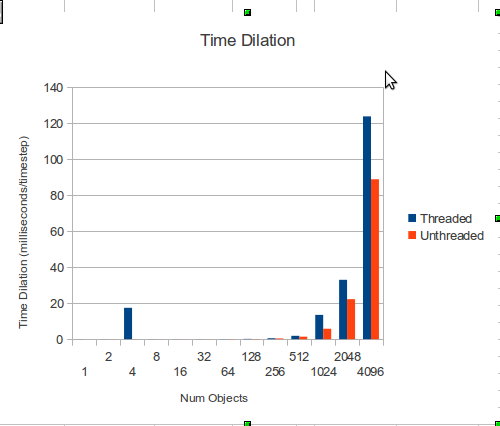
\includegraphics[width=.45\textwidth]{plot.png}
	\captionof{figure}{Performance Data}
	\label{fig:data}
\end{center}

\section{Conclusion} 


As we have only completed the preliminary set of data gathering, and have not implemented our predictive algorithm, we are not able to draw any conclusions as of yet.  Upon completion of the predictive algorithm implementation, and the subsequent data gathering and analysis, we will be able to form appropriate conclusions.

\bibliographystyle{IEEEtran}
\bibliography{IEEEabrv,midterm}

\appendix %Steven
\section{Project Progress}
This project is progressing well.  Save several hiccups in the implementation, we now have a very large and stable mature codebase that implements the naive implementations of the algorithm and allows
us to visualize the result.
\subsection{Challenges Encountered}
We encountered several challenges when implementing this project.  Although the simulation algorithm is simple in theory, debugging and implementing the physics behind the spheres caused a few small problems we did not foresee.

\subsubsection{Visualizer}
We had a great deal of small bugs that needed to be solved.  The primary method of solving this problem from a debugging perspective was the implementation of a real-time visualization in OpenGL.
This visualization was a little slow, but it facilitated debugging of our simulation.  Creating this visualization required some tweaking of the core simulator to allow a callback hook, as well as some OpenGL code to render the spheres in real-time.

\begin{center}
	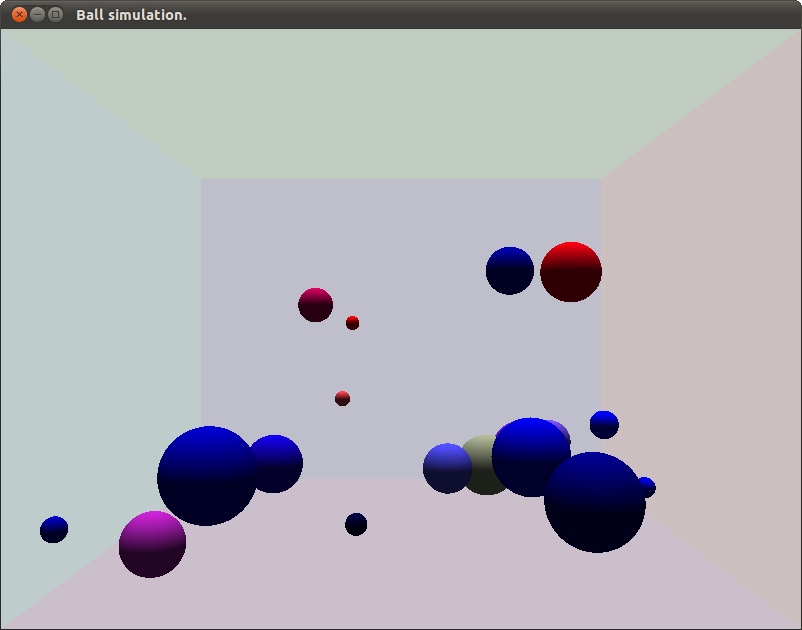
\includegraphics[width=.45\textwidth]{few.png}
	\captionof{figure}{A few balls}
	\label{fig:few}
\end{center}

\begin{center}
	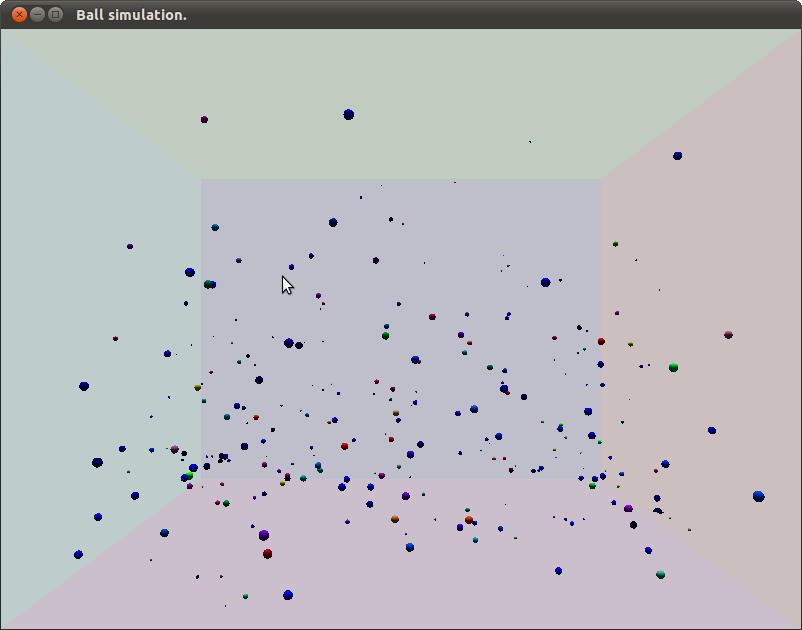
\includegraphics[width=.45\textwidth]{lots.png}
	\captionof{figure}{Lots of balls}
	\label{fig:lots}
\end{center}

\subsubsection{Sticky Spheres}
At our first running of the algorithm, we noticed that the number of registered sphere-sphere collisions was greater than the number of timesteps.  This should be impossible, as a sphere-sphere collision should
occur very rarely, depending on the total volume of the space and the number of spheres in the simulation.  Even when the number of spheres was 2, this phenomena occured.  Upon debugging the simulation with the visualizer,
we observed that any time a sphere collided with a larger sphere, it immediately became stuck inside the larger one, as shown in \ref{fig:linked}.  

\begin{center}
	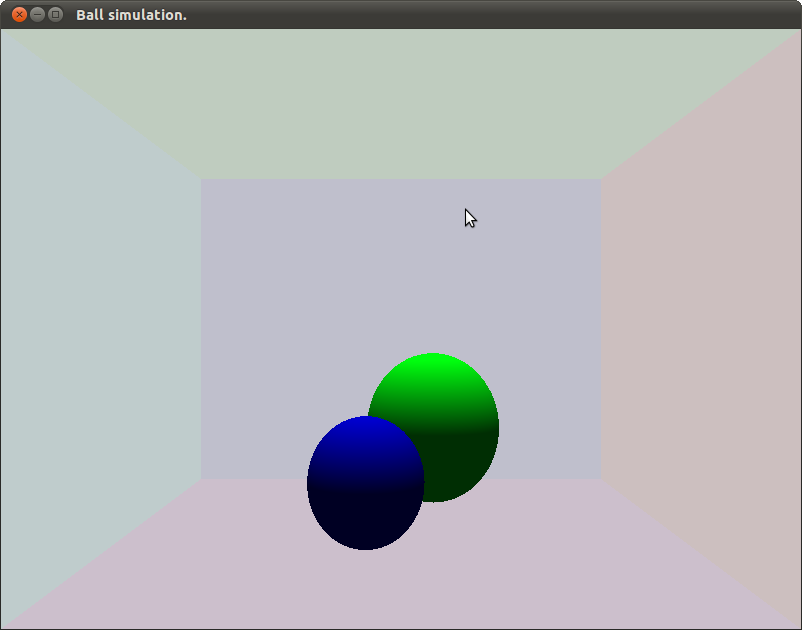
\includegraphics[width=.45\textwidth]{linked.png}
	\captionof{figure}{Two Linked Spheres}
	\label{fig:linked}
\end{center}

This problem generated 1 sphere-sphere collisions for each frame, for each pair of 'stuck' spheres.  To mitigate this problem, we implemented a simple hack that pushed the spheres away from each other by a distance equal to the sum of their radii plus an epsilon.
This dramatically reduced the number of sphere-sphere collisions to the correct number.

\subsubsection{Thread Overhead}
	Our implementation of the threading uses the OpenMP compiler extension subsystem.  Our implementation, which is a part of gcc 4.5, is built on top of pthreads under linux.  In our implementation, we 
spawn a number of worker threads per timestamp in order to thread the system.  Our implementation of the naive algorithm should scale linearly with the number of threads.  However, in our implementation this is not the case.  We strongly suspect that
several factors could be contributing to this difficulty.  

\begin{itemize}
	\item The overhead of spawning multiple threads per timestep dwarfs the work done by the update step
	\item The thread spawn behavior is sub-optimal as described by \cite{performance-critical}
	\item Thread affinity is poor.
	\item Threads may be competing for the global statistical variables we are using to measure performance.
\end{itemize}

We intend on investigating all of these possibilities immediately in the following weeks.  It is important to do so, because our argument for the applicability of this algorithm to parallel data-structures
is based on the necessity of competing with the highly-scalable naive algorithm.  If we fail to implement a scalable naive algorithm, then our ability to implement a scalable predictive algorithm is questionable.

\subsection{Completed Tasks}
\subsubsection{Simulation Framework}
We completed a simulation framework capable of interactively running our simulation in multiple different configurations from the command line.  Our simulation framework correctly
creates a simulation in a memory and cpu-efficiant way, and allows us to extend the implementation of the update step without changing the rest of the codebase.
\subsubsection{Visualization Framework}
In order to debug and to visualize the state of the simulation at a given timestep, a visualization in opengl was produced.
\subsubsection{Threaded and Non-Threaded Naive Implementation}
The implementation of our Naive algorithm is complete for the threaded and the non-threaded implementation.  However, as previously described, our implementation does not scale.  However, it is verified to function
correctly in both implementatons.

\subsection{Remaining Tasks}
There are 3 major tasks remaining.
\begin{itemize}
\item Fix the scalability of the naive algorithm and generate new data.
\item Write the predictive algorithm and test.
\item Finish the final report.
\end{itemize}

\subsection{Target Conference}
Currently, we would like to aim for a submission to the IEEE IPDPS Symposium (\url{http://ieeexplore.ieee.org/xpl/mostRecentIssue.jsp?punumber=5136864}).  In order to prepare for this submission, much additional research will be needed, with more detailed and robust follow up experimentation.  This experimentation will include, but not be limited to:
\begin{itemize}
\item implementation of the semi-naive algorithm,
\item robust and accurate physics calculations,
\item bug-free code base, and
\item more robust test cases.
\end{itemize}

% An example of a floating figure using the graphicx package.
% Note that \label must occur AFTER (or within) \caption.
% For figures, \caption should occur after the \includegraphics.
% Note that IEEEtran v1.7 and later has special internal code that
% is designed to preserve the operation of \label within \caption
% even when the captionsoff option is in effect. However, because
% of issues like this, it may be the safest practice to put all your
% \label just after \caption rather than within \caption{}.
%
% Reminder: the "draftcls" or "draftclsnofoot", not "draft", class
% option should be used if it is desired that the figures are to be
% displayed while in draft mode.
%
%\begin{figure}[!t]
%\centering
%\includegraphics[width=2.5in]{myfigure}
% where an .eps filename suffix will be assumed under latex, 
% and a .pdf suffix will be assumed for pdflatex; or what has been declared
% via \DeclareGraphicsExtensions.
%\caption{Simulation Results}
%\label{fig_sim}
%\end{figure}

% Note that IEEE typically puts floats only at the top, even when this
% results in a large percentage of a column being occupied by floats.


% An example of a double column floating figure using two subfigures.
% (The subfig.sty package must be loaded for this to work.)
% The subfigure \label commands are set within each subfloat command, the
% \label for the overall figure must come after \caption.
% \hfil must be used as a separator to get equal spacing.
% The subfigure.sty package works much the same way, except \subfigure is
% used instead of \subfloat.
%
%\begin{figure*}[!t]
%\centerline{\subfloat[Case I]\includegraphics[width=2.5in]{subfigcase1}%
%\label{fig_first_case}}
%\hfil
%\subfloat[Case II]{\includegraphics[width=2.5in]{subfigcase2}%
%\label{fig_second_case}}}
%\caption{Simulation results}
%\label{fig_sim}
%\end{figure*}
%
% Note that often IEEE papers with subfigures do not employ subfigure
% captions (using the optional argument to \subfloat), but instead will
% reference/describe all of them (a), (b), etc., within the main caption.


% An example of a floating table. Note that, for IEEE style tables, the 
% \caption command should come BEFORE the table. Table text will default to
% \footnotesize as IEEE normally uses this smaller font for tables.
% The \label must come after \caption as always.
%
%\begin{table}[!t]
%% increase table row spacing, adjust to taste
%\renewcommand{\arraystretch}{1.3}
% if using array.sty, it might be a good idea to tweak the value of
% \extrarowheight as needed to properly center the text within the cells
%\caption{An Example of a Table}
%\label{table_example}
%\centering
%% Some packages, such as MDW tools, offer better commands for making tables
%% than the plain LaTeX2e tabular which is used here.
%\begin{tabular}{|c||c|}
%\hline
%One & Two\\
%\hline
%Three & Four\\
%\hline
%\end{tabular}
%\end{table}


% Note that IEEE does not put floats in the very first column - or typically
% anywhere on the first page for that matter. Also, in-text middle ("here")
% positioning is not used. Most IEEE journals/conferences use top floats
% exclusively. Note that, LaTeX2e, unlike IEEE journals/conferences, places
% footnotes above bottom floats. This can be corrected via the \fnbelowfloat
% command of the stfloats package.


% trigger a \newpage just before the given reference
% number - used to balance the columns on the last page
% adjust value as needed - may need to be readjusted if
% the document is modified later
%\IEEEtriggeratref{8}
% The "triggered" command can be changed if desired:
%\IEEEtriggercmd{\enlargethispage{-5in}}

% references section

% can use a bibliography generated by BibTeX as a .bbl file
% BibTeX documentation can be easily obtained at:
% http://www.ctan.org/tex-archive/biblio/bibtex/contrib/doc/
% The IEEEtran BibTeX style support page is at:
% http://www.michaelshell.org/tex/ieeetran/bibtex/
%\bibliographystyle{IEEEtran}
% argument is your BibTeX string definitions and bibliography database(s)
%\bibliography{IEEEabrv,midterm.bib}
%
% <OR> manually copy in the resultant .bbl file
% set second argument of \begin to the number of references
% (used to reserve space for the reference number labels box)

%\begin{thebibliography}{1}

%\bibitem{IEEEhowto:kopka}
%H.~Kopka and P.~W. Daly, \emph{A Guide to \LaTeX}, 3rd~ed.\hskip 1em plus
%  0.5em minus 0.4em\relax Harlow, England: Addison-Wesley, 1999.

%\end{thebibliography}

%\bibliographystyle{ieeetr}
%\bibliography{midterm}

%\appendix
%\section{Project Progress}
%\subsection{Challenges Encountered}
%\subsection{Completed Tasks}
%\subsection{Remaining Tasks}


% that's all folks
%\bibliographystyle{ieeetr}
%\bibliography{midterm}




%\appendix
%\section{Project Progress}
%\subsection{Challenges Encountered}
%\subsection{Completed Tasks}
%\subsection{Remaining Tasks}

\end{document}


